\newcommand{\pwd}{key}

\renewcommand{\password}{key\xspace}

We introduce the problem  through an example, and outline our
approach.  We work with a  small, class-based object-oriented, \se{sequential} language similar to Joe-E \cite{JoeE} with modules,   module-private fields
({accessible} only from   methods {from} the same module),
% not that central, we dicuss this later %initalised by a class's implicit constructor, 
and unforgeable, un-enumerable addresses.
We distinguish between  \emph{\internalO}
objects --- instances of our internal module $M$'s classes ---
and \emph{\externalO} objects defined in
\emph{any} number of external modules $\overline M$.~ 
{\prg{Private} methods  {may only be} called by objects of the same
  module,  while \prg{public}  methods  may be called by \emph{any}
  object with a reference to the method receiver, {and with
  actual arguments of  dynamic types that match} the declared formal parameter types.} 
% SD dropped
% Our model of execution is entirely unsurprising with a stack, a heap, and states.
\footnote{As in Joe-E, we leverage  module-based privacy to restrict propagation of capabilities, and reduce the need for reference monitors etc, \cf Sect 3 in  \cite{JoeE}.}   

% \subsubsection{Internal and external modules, objects, and states}
 \label{s:concepts}

We are concerned with guarantees made in an \emph{open} setting; that
is, our internal module
$M$ must be programmed so that 
its execution, together with any external modules $\overline M$
will satisfy these guarantees.
$M$ must ensure these guarantees are satisfied
whenever the
$\overline M$  \emph{\externalM} modules are executing,
yet without relying on any assumptions about $\overline M$'s code
(beyond the programming language's semantics)%
\footnote{
This is a critical distinction from e.g.\
cooperative approaches such as rely/guarantee
\cite{relyGuarantee-HayesJones-setss2017,relyGuarantee-vanStaden-mpc2015}.}.
The internal module may break these guarantees temporarily,
so long as they {are reestablished} before (re)entry to an external module.
 

% \kjx{haven't mentioned states yet, so this is too early --- We also distinguish between
%      \emph{\internalC} and   \emph{\externalC} states - those whose receiver is internal or external respectively. }
 
 

\subsection*{\prg{Shop} -- illustrating tamed effects} % Reason about external calls (using protection)}
\label{sec:how}
\label{sec:shop}

The challenge when calling a method on an external object, is that we have no specification for that method. 
 For illustration, consider the following, internal, module \Mshop, which also includes the classes \prg{Item}, \prg{Shop}, \prg{Account}, and \prg{Inventory}. 
Classes  {\prg{Inventory} and \prg{Item} have the expected functionality. 
\prg{Account}s hold a balance and have a \password. 
With access to an \prg{Account}, %'s address, 
one  can pay money into it, 
and with access to an account  and its \password, one can withdraw money from it.
Implementations of such a class  appear in the next section.
}
 \prg{Shop}  has  a public method \prg{buy} whose formal parameter \prg{buyer} is an \prg{external}   object. 
 % SD chopped  with a method { \prg{pay}.}} 

\begin{lstlisting}[mathescape=true, language=Chainmail, frame=lines]
module M$_{shop}$
  ...   
  class Shop
    field accnt:Account, invntry:Inventory, clients:external      
    public method buy(buyer:external, anItem:Item)
      int price = anItem.price
      int oldBlnce = this.accnt.blnce
      buyer.pay(this.accnt, price)     // $\red{\mbox{external\ call}}$
      if (this.accnt.blnce == oldBlnce+price)  
         this.send(buyer,anItem)
      else
         buyer.tell("you have not paid me")      
    private method send(buyer:external, anItem:Item)  
       ...         
\end{lstlisting}
 

The critical point is the external call on line 8,   {where the \prg{Shop} asks the \prg{buyer} to pay the price of that item,
by calling  \prg{pay} on \prg{buyer} and passing the \prg{Shop} account as an argument.
As \prg{buyer} is an external object, the module \Mshop has no method specification for \prg{pay}, and no 
certainty about what its implementation %knowledge of what the implementation of \prg{pay} 
might do. 
% \se{with \prg{this.accnt}}. 
% but also with other things.
}

{What are the possible effects of that external call?}
% How can we reason about this external call?
{The \prg{Shop} hopes, but cannot be sure, that at line 9  it  will have received money; but 
it wants to be certain  that the \prg{buyer} can not use this opportunity to access the 
shop's account to drain its money.
Can \prg{Shop}  be certain?}

\vspace{.05cm}
% \noindent
%Indeed, if \Mshop  makes appropriate guarantees, it can \tame  the effects at line 8. In particular,  
% \\
%$\strut \ \ \ (A)\ \ $ If  \prg{buyer} \sdN{did not have eventual access to the account's \password before the call of  \prg{buy}} \ \ \    {\emph{ and}}  \\
%$\strut \ \ \ (B)\ \ $ If \Mshop guarantees that a) keys do not get leaked to external objects, and b) no money can be withdrawn % from an account 
%unless the external\\  
%$\strut \ \ \ \ \ \ \ \ \ \ \ $ object causing the withdrawal can eventually get access to the account's \password, \ \ \  {\emph{then}} \\
%$\strut \ \ \ (C)\ \ $ The external  call on line 8 will not cause a reduction in the shop's account's balance.
\begin{enumerate}[(A)]
\item   If prior to the call of  \prg{buy}, the \prg{buyer}  has no eventual access to the account's \password, \ \ \ \emph{----} and
\item  If \Mshop ensures that a) access to keys is not leaked to external objects, 
and b) funds cannot be withdrawn unless the external entity responsible for the withdrawal has eventual access to the account's \password, \ \ \ \emph{----} then
\item  The external  call on line 8 will not result  in a decrease in the shop's account balance.
\end{enumerate}

%\vspace{.3cm}
\noindent
The remit of this paper is to provide specification and verification tools that support arguments like the one above. In that example, we relied on two yet-to-be-defined concepts: (1) ``eventual access'' and (2) \tamed effects (e.g., no money withdrawn unless certain conditions are met).
%We need to define these concepts, and develop Hoare Logics for reasoning.
Therefore, we need to address the following three challenges: 
\begin{description}
\item[\ \ \ \ \  1$^{st}$ Challenge] The specification   of ``eventual  access''. 

\item[\ \ \ \ \   2$^{nd}$ Challenge] The specification of tamed effects, 

\item[\ \ \ \ \  3$^{rd}$ Challenge] A  Hoare Logic for external calls, and for adherence to tamed effect specifications.
\end{description}
%
%\vspace{.2cm}
%\noindent
% \textbf{NOTE}  \sdN{Replacing the argument by a wrapper to the account which allows payments but forbids withdrawals,    would be ineffectual in \taming} the  effects on line 9. 
%What  if the % nece\tame the effects because
% \prg{buyer} had access to the account and its \password  \emph{before} the call to \prg{pay}? 
%\se{I don't understand the point here. Are you saying a wrapper might prevent a buyer who has legitimate access to an account from getting it?}
%\sdN{SD: The point I am trying to make is that: \  if before the call to \prg{pay}, the \prg{buyer} had access to the account and its keyword, and when we call \prg{pay} instead of 
%\prg{this.accnt} we pass the wrapper, then the \prg{buyer} would still be able to steal money from \prg{this.accnt}.
%Does this make sense? Shall we drop that point?}
 
 
\subsection{1$^{st}$ Challenge: eventual access} 


Assume we have a guarantee that no external object $o_e$ can cause an effect $E$ unless it has direct access to the capability object $o_{cap}$. To ensure $o_e$ will not cause $E$, we must ensure that $o_e$ not only lacks access now but also cannot gain access in the future.  We call this  ``lack of eventual access.''

We approximate ``lack of eventual access'' through \emph{protection}, defined befow, and illustrated in %illustrated in Figure
Fig.  \ref{fig:ProtectedBoth}.  %
%We propose the concept of \emph{protection} to describe absence of eventual access. 
%%An object $o$ is  \emph{protected} if external objects cannot directly access $o$ unless this access is granted by an internal object.
%An object   is   \emph{protected} if it remains inaccessible to external objects unless an internal object explicitly grants access.

 \begin{description}
\item[Protection] Object $o$ is \emph{protected  from} $o'$, formally $\protectedFrom {o} {o'}$,  
 if the penultimate object on \se{every} path from $o$ to $o'$  is internal.
Object $o$ is \emph{protected}, formally ${\inside{\prg{\it{o}}}}$, if $o$ is protected from all external objects transitively accessible from the currently executing method call. %More in 
-- \cf \susan{Def. \ref{def:chainmail-protection-from}}. % and 

 \end{description}
 
 % if $o'$ cannot obtain direct access to $o$ unless an internal object affords that access. %to $o$. 

 %{Program execution may turn protected objects to un-protected, but this may only be caused by execution of an internal method -- hence only internal objects can afford that access.}

If the  internal module  never passes $o$ to any external object (\ie never leaks $o$,) then if $o$ is protected from $o_e$ now, it will remain protected from $o_e$,
and if $o$ is protected now, it will remain protected.
Going back to the original question, if $o_e$ is protected from all locally accessible external objects, effect  $E$ is guaranteed not to occur, \se{unless caused by internal code}.

\begin{figure}[tbh]
\begin{tabular}{|c|c|c|}
\hline
\resizebox{3.5cm}{!}{
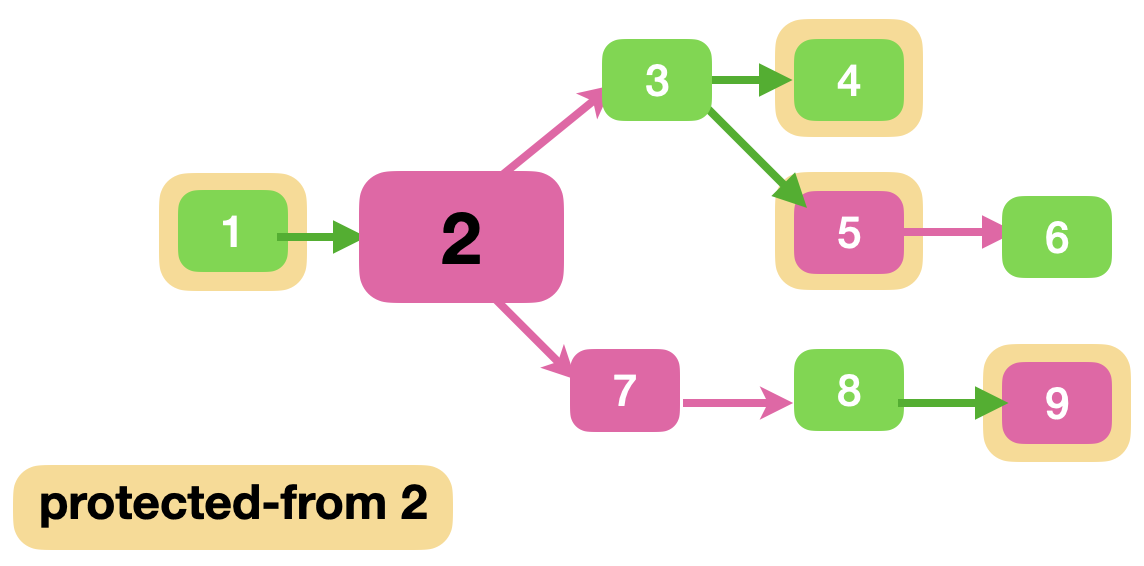
\includegraphics[width=\linewidth]{diagrams/prfC.png}
} 
&
\resizebox{4.5cm}{!}{
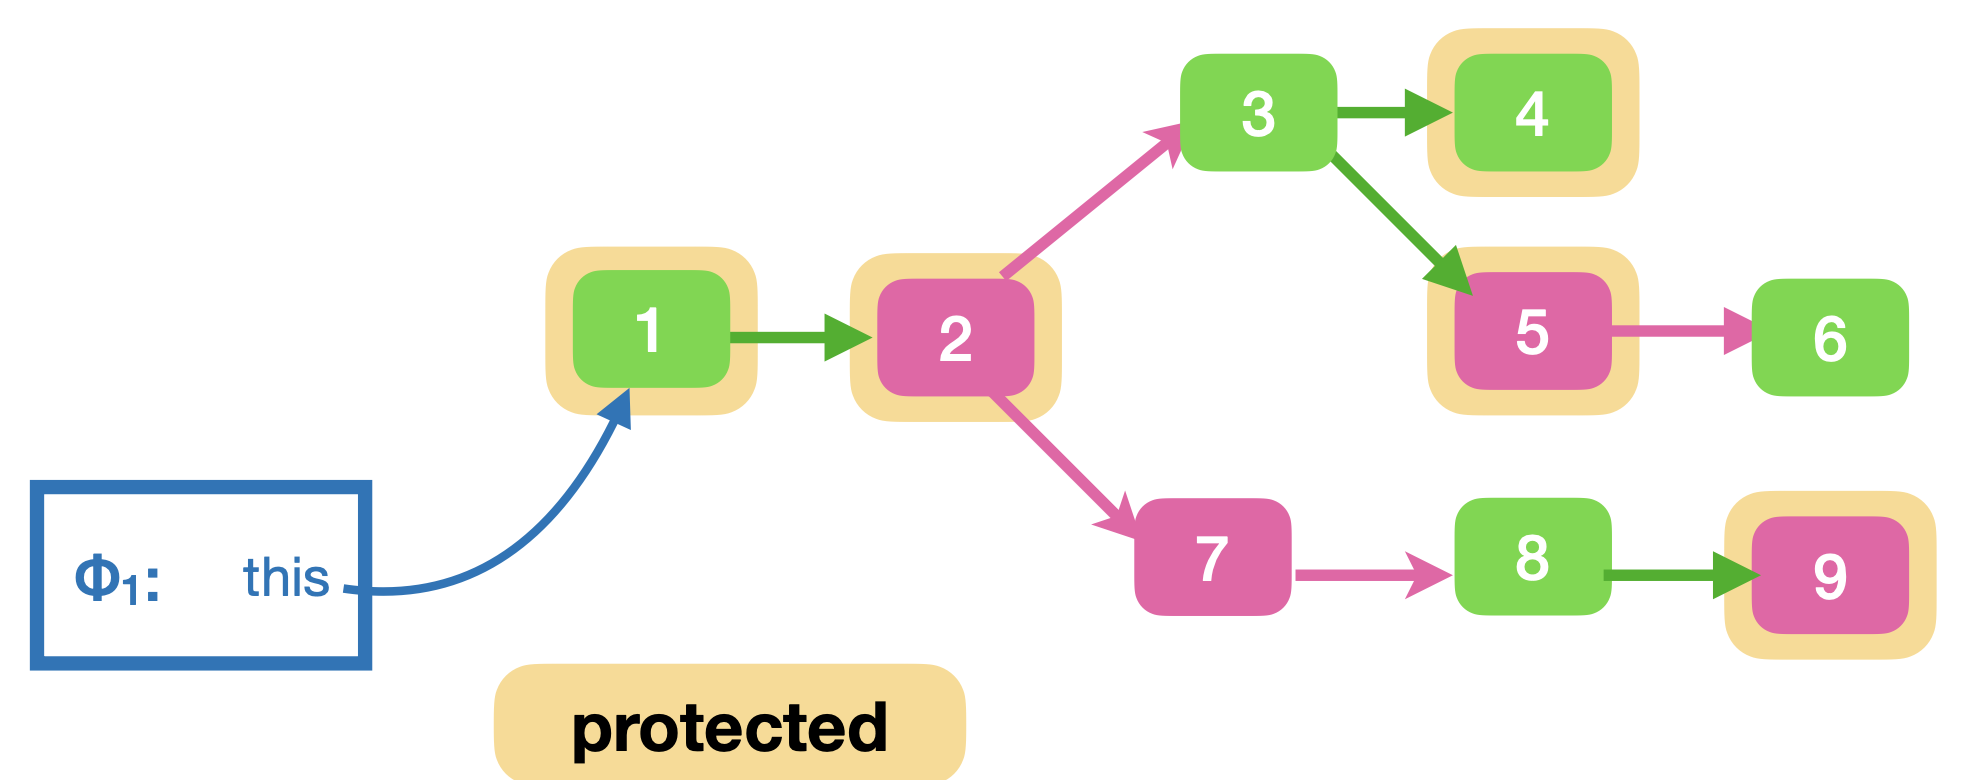
\includegraphics[width=\linewidth]{diagrams/prtFirst.png}
}
&
\resizebox{4.5cm}{!}{
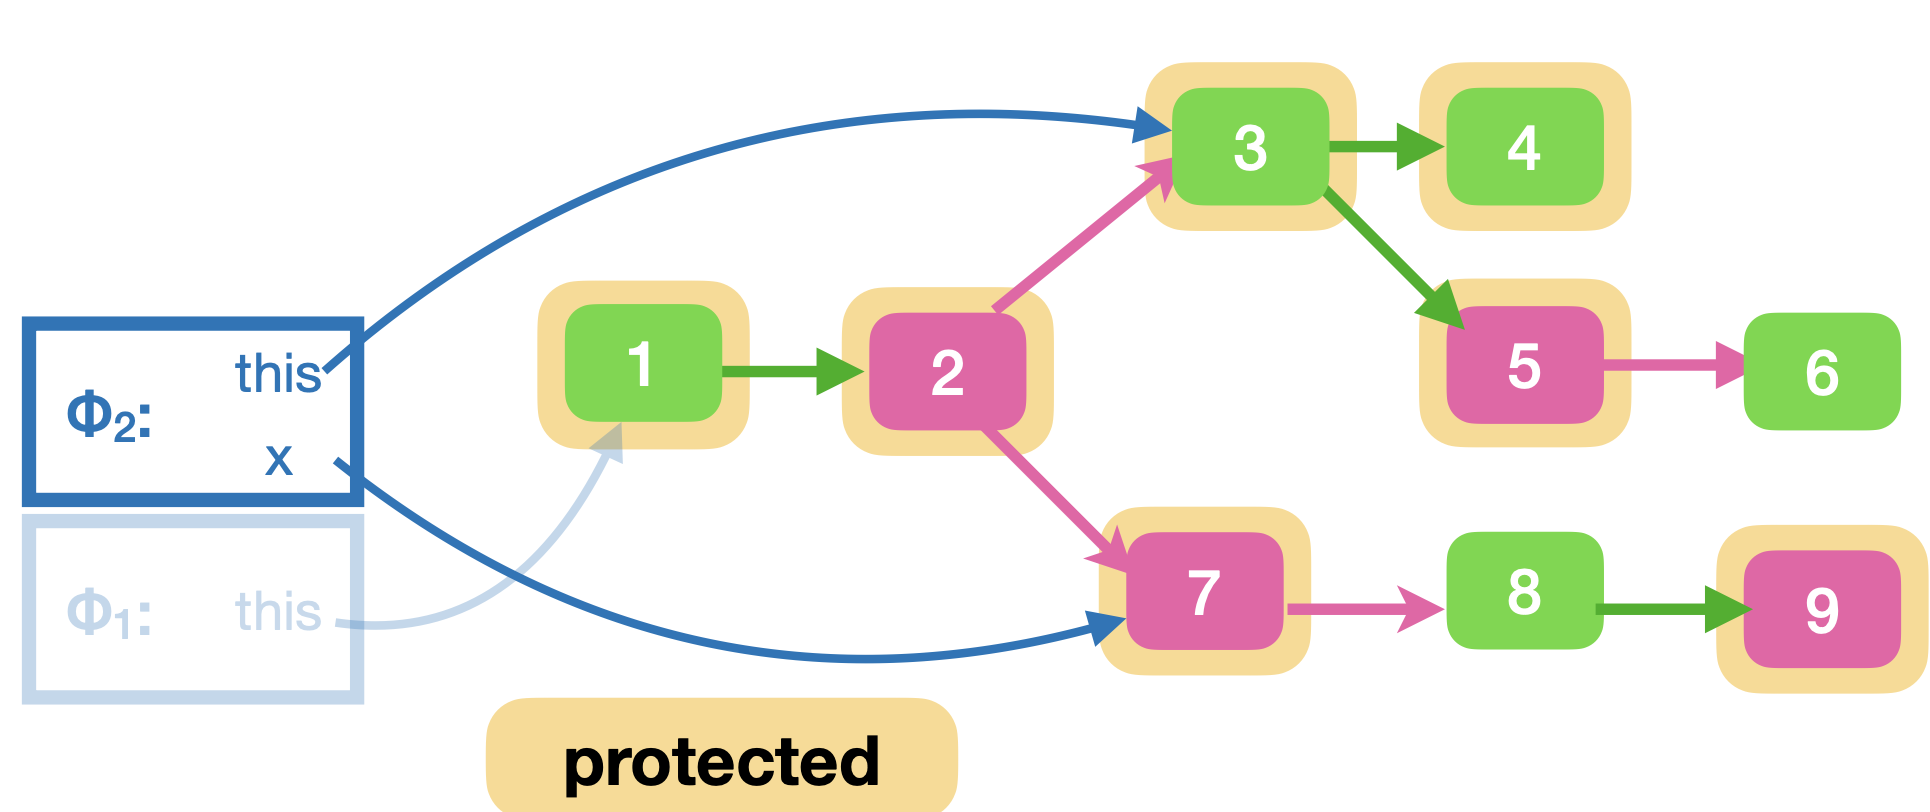
\includegraphics[width=\linewidth]{diagrams/prtSecond.png}
}
\\
\hline
protected from object $o_2$
&
protected  with top frame $\phi_1$
&
protected  with top frame $\phi_2$
\\
\hline \hline
\end{tabular}
\caption{Protected from and Protected. Pink and green squares are external and internal objects, respectively. Connecting straight arrows  indicate fields. Blue boxes are frames on the stack. Protected objects are  highlighted in yellow. 
 The left pane shows a heap with objects $o_1$-$o_9$.
 Here  $o_1$, $o_4$, $o_5$ and $o_9$ 
are protected from $o_2$. 
 The middle pane {shows the same heap and a stack with frame  $\phi_1$} whose receiver,   \prg{this},  points to $o_1$. Here 
 $o_1$, $o_2$, $o_4$, $o_5$ and $o_9$  are protected. 
 The right pane {shows the same configuration, but after pushing frame  $\phi_2$}, whose receiver,  \prg{this},  and local variable, \prg{x}, point to $o_3$ and  $o_7$, respectively.
 Here $o_3$ and $o_7$ are protected, in addition  to  the objects protected in the previous pane.
}
   \label{fig:ProtectedBoth}
 \end{figure}
 

\subsection{2$^{nd}$ Challenge: Specification of tamed effects}
\label{sect:approach:scoped}
How can we express the guarantee that effects are \tamed?  
 In particular, when effects can be the outcome of the execution of more than one method? 
 Traditional,  {per-method} PRE/POST conditions {cannot guarantee} %specifications cannot express guarantees
  that two or more of our methods won't interact to produce an untamed effect. 
We build on the concept of history invariants \cite{liskov94behavioral,usinghistory,Cohen10} and define

\begin{description}
\item[{Scoped invariants}]  
{$\TwoStatesN  {\overline{x:C}}  {A}$} expresses that if a {state} $\sigma$ 
 has objects $\overline x$ of class $\overline C$, and satisfies $A$, then all $\sigma$'s \emph{scoped  future  states} will  {also} satisfy  {$A$}. 
The scoped future contains all % \sdN{future} 
 states which can be reached through any steps, including further method calls and returns, but stopping before returning  from the call active in $\sigma$ \footnote{{Here lies the difference to history invariants, which consider \emph{all} future states, including returning from the call active in $\sigma$.}}  --  \cf Def  \ref{def:shallow:term}.
{For} $\sigma$ and its scoped future   we only consider external states -- \cf Def \ref{def:necessity-semantics}.
\end{description}

    
\label{s:bank}



\begin{example}
\label{s:bankSpecEx}
The following scoped invariants\\
$\strut \SPSP\ \ \   S_1\ \  \triangleq \ \ \TwoStatesN {\prg{a}:\prg{Account}}  {\inside{\prg{a}}} $ 
\hspace{1.1cm}
$\strut  \SPSP\ \ \   S_2\ \  \triangleq \ \ \TwoStatesN  {\prg{a}:\prg{Account}}  {\inside{\prg{a.key}}} $ 
% \\
%$\strut  \SPSP   S_3\ \  \triangleq \ \ \TwoStatesN {\prg{a}:\prg{Account},\prg{b}:\prg{int}}  {\inside{\prg{a}} \wedge \prg{a.\balance}=\prg{b}}  $
\\
$\strut  \SPSP\ \ \   S_3\ \  \triangleq \ \ \TwoStatesN{ \prg{a}:\prg{Account},\prg{b}:\prg{int} } {\inside{\prg{a.key}} \wedge \prg{a.\balance} \geq \prg{b} } $ 
% \end{tabular}
%}

\noindent
%specifications
 guarantee that   accounts are not leaked  ($S_1$), \ \ keys are not leaked  ($S_2$), \ \ the balance does not decrease unless there is unprotected access to the key  ($S_3$).
 % $\strut  \SPSP  S_1$:\   accounts are not leaked,  \hspace{1.1cm}
%$\strut   \SPSP S_2$:\    keys are not leaked,\\
%%$\strut \SPSP  S_3$:\  the balance is not modified unless there is unprotected access to the account,  \\%while 
%$\strut \SPSP  S_3$:\   the balance does not decrease unless there is unprotected access to the key.  
%
\end{example} 


 
 \vspace{.05cm}

 
\noindent
{\textbf{\sdN{Scoped invariants are} \emph{conditional}}:}  They ensure that assertions are \emph{preserved}, but unlike object invariants, they do not guarantee that they always hold.
\ \Eg   \prg{buy} cannot assume $\inside{a.\prg{key}}$ holds on entry, but   guarantees that if it holds on entry, then  it will still hold on exit.

 
 \begin{example}
 We   use the features from the previous section to specify methods. 

{\sprepost
		{\strut \ \ \ \ S_4} 
		{   \protectedFrom{\prg{this}.\prg{\myAccount}.\prg{key}} {\prg{buyer}} \wedge \prg{this}.\prg{\myAccount}.\prg{\balance}=b
		 }
		{\prg{public Shop}} {\prg{buy}} {\prg{buyer}:\prg{external}, \prg{anItem}:\prg{Item} }
		{ 
		  %\protectedFrom{\prg{this}.\prg{\myAccount}.\prg{key}} {\prg{buyer}} \wedge 
		  \prg{this}.\prg{\myAccount}.\prg{\balance}\geq b
		 }
}

\noindent
$S_4$  guarantees that if the % account's 
key was protected from \prg{buyer} before the call, then the balance will not decrease. %SD is shorter, but I hope ckear eniugh  \prg{buy} will not decrease the %shop's account  balance. 
 It does \emph{not} guarantee \prg{buy} will only be called when $\protectedFrom{\prg{this}.\prg{\myAccount}.\prg{key}} {\prg{buyer}}$ holds. 
As a  public method,  \prg{buy}  can be invoked by external code that ignores all specifications.
\end{example}

% \vspace{.05cm}

\begin{example}
We illustrate the meaning of our specifications  using three  versions of a class \prg{Account}  from  \cite{OOPSLA22} 
as part of our internal module \Mshop. 
To differentiate, we rename \Mshop  as $\ModA$,  $\ModB$, or $\ModC$. 
All use the same \prg{transfer} method for withdrawing money.
%All use the same method \prg{transfer} to  withdraw money, only when supplied with the key.
%\forget{All versions {use the same method \prg{transfer} to} allow  withdrawal of money, only when supplied with the key to the account.
%All use the same method \prg{transfer} to  withdraw money, only when supplied with the key.}
% removed class Key -- it does not need to be internal 
\begin{lstlisting}[mathescape=true, language=Chainmail, frame=lines]
module $\ModA$      
  class Shop   ... as earlier ...
  class Account
    field blnce:int 
    field key:Key
    public method transfer(dest:Account, key':Key, amt:int)
       if (this.key==key')   this.blnce-=amt; dest.blnce+=amt
     public method set(key':Key)
       if (this.key==null)  this.key=key'
\end{lstlisting}

Now consider  modules \ModB and \ModC which differ from \ModA only in their \prg{set} methods. Whereas \ModA 's key is immutable, \ModB allows any client to reset an account's key at any time, and \ModC requires the existing key in order to change it.
  

\begin{tabular}{lll}
\begin{minipage}[b]{0.40\textwidth}

\begin{lstlisting}[mathescape=true, language=Chainmail, frame=lines]
$\ModB$
public method set(key':Key)
  this.key=key'
\end{lstlisting}
\end{minipage}
&\ \ \  \ \   &%
\begin{minipage}[b]{0.48\textwidth}
\begin{lstlisting}[mathescape=true, language=chainmail, frame=lines]
$\ModC$
public method set(key',key'':Key)
  if (this.key==key')  this.key=key''
\end{lstlisting}
\end{minipage} 
\end{tabular}

{Thus, in all three modules, the key is a capability which \emph{enables} the withdrawal of the money. 
Moreover, in $\ModA$ and $\ModC$, the key
{is a capability} used to  \emph{tame} withdrawal of money, preventing those without it from getting the money from the account.}
Crucially,  in $\ModB$ the key \emph{does not tame} withdrawal of money.
Using $\ModB$, it is possible to start in a state where the account's key is unknown, modify the key, and then withdraw the money. 
Code  {such as}
\\ 
$\ \strut \hspace{.2in} $ \prg{k=new Key;  acc.set(k); acc.transfer(rogue\_accnt,k,1000)} 
\\ 
is enough to drain  \prg{acc} in \ModB without knowing the \password.\footnoteSD{CAREFUL: we had 
$\ \strut \hspace{.01in} $ \prg{an\_account.set(42); an\_account.transfer(rogue\_accnt,42)} but this was type incorrect!}
 %
% \emph{Emergent behaviour} is key here: 
Even though % the method 
\prg{transfer} in  \ModB is ``safe'' when considered in isolation, it is not safe when considered in conjunction with other methods from the same module. 

Modules $\ModA$ and $\ModC$ satisfy $S_2$ and $S_3$, while $\ModB$ satisfies neither. No module can satisfy $S_1$. 
\end{example}
 
\forget{% for the time being at least
{ \noindent
 Our specifications are  in terms of the complete module, rather than per-method.
 They talk about externally observable effects (\eg the key stays protected), 
 % the account's balance may increase), 
 rather than about  individual methods (\eg\, \prg{set}). %  or \prg{transfer}).
{Thus,   they can characterize  any 
module with  accounts which have a % {\textit{implementation}} of a bank account with a 
 \balance~and a \password -- even as ghost fields --}  irrespective of the API offered.
} }% , services  exported, or  dependencies on other parts of the system.\footnoteSD{does this come from OOPSLA? if so we need to rephrase}
%\notesep
%Adherence to   specifications is not monotonic:
%{Eg, while  \ModA satisfies $S_3$, the addition of \prg{set} lead to \ModB, which does not.}
%% Adding a method to a module does not necessarily preserve such adherence,
%% \eg adding method \prg{set} in module \ModB breaks 
%%SD removed the below. When we changed the invaraints to have the same assertion re and post it no longer hel
%\forget{, and while separate methods may adhere to a  specification, their combination does
%not necessarily do so. 
%{For example, \ModB's  \prg{tansfer} and \prg{set} satisfy $S_3$, but their interplay does not.}
%%In this sense, and, similar to OOPSLA'22, our  specifications capture a module's \emph{emergent behaviour}. 


  
  \subsection{3$^{rd}$ Challenge:  A Hoare logic} %  for external calls} %  (using scoped invariants)}
 \label{sec:howThird}


 
 \vspace{.1cm}
 
We now move to the  verification of $S_4$. 
The challenge is how to reason  about the external call on line 8. %, even though we do not have a specification for \prg{pay}
% the  {called method}, we know that the effects of the call are tamed according to the module's scoped invariants. 
% SD BELOW is wrong. left just in case we want to adapt ir.
% That is expressed in the  simplified Hoare rule below -- \cf. Fig.\ref{f:external:calls}. 
% 
%  $\inferruleNoName  
% 	{ 
%   	   {\TwoStatesN {\overline {x:D}} {A}}\ \   \mbox{is part of $M$'s specification}
%        }
%	{   \triple { \    { \external{y_0}} \,     \wedge \,  \overline{x:D}\  \wedge\  A\ }  
%						{ \ u:=y_0.m(y_1,.. y_n)\    }
%						{ \    A  \ }
%						\  \  ...
%         }
%$
%
%\vspace{.05cm}
% 
% Now  revisit the external call from line 9 in Section \ref{sec:shop}. Our argument is that 
We aim to establish a Hoare triple of the form:
 \\
$\strut \ \ \ \ \ \ \ \ \ \ \  \{\  \ { \external{\prg{buyer}}} \ \wedge\ {\protectedFrom {\prg{this.\myAccount.key}} {\prg{buyer}}\ \wedge\ {\prg{this.\myAccount.\balance}}= b    }\ \  \}$\\
$\strut \ \ \ \ \ \ \ \ \ \ \   \ \ \ \ \ \ \ \ \ \ \ \ {\ \prg{buyer.pay(this.accnt,price)}   \ } $\\
$\strut \ \ \ \ \ \ \ \ \ \ \  \{\  \ \  {\prg{this.\myAccount.\balance}} \geq  b \  \  \}$ 
\\
The intuitive reasoning is as follows: if the shop's account's key is protected from \prg{buyer} (A from earlier), and the module satisfies $S_3$ (B), then after the call, the account's balance will not decrease (C).
%
However, application of $S_3$ is not straightforward. 
%While $S_3$ preserves ${\inside{\prg{a.key}}} \wedge ...$,
%Application of $S_3$ 
It requires ${\inside{\prg{a.key}}} \wedge ...$,  but  the call's precondition only guarantees $\protectedFrom{\prg{this.\myAccount.key}}{\prg{buyer}}$. 
%To apply $S_3$, we would need to know ${\inside{\prg{this.\myAccount.key}}}$, but we only know $\protectedFrom{\prg{this.\myAccount.key}}{\prg{buyer}}$.


%, while we  need the stronger property  ${\inside {\prg{this.\myAccount.key}}}$. 

While we do not know whether \prg{a.key} is protected during  execution of \prg{buy}\footnote{For instance, one of the clients may have access to it.}, we can be certain it is protected during execution of \prg{pay}.  This is so, because the objects accessible during \prg{pay} are those visible from its arguments (\ie \prg{buyer} and \prg{price}).
% \footnote{Generally, more objects are protected from the viewpoint of the called function than from that of the caller -- \cf  Fig. \ref{fig},}

%To express this difference, 
We define the adaptation operator $\FIXSymbolA$, which translates an assertion from the viewpoint of the called function to that of the caller. 
Specifically, $\PushAS y A$ ensures that $A$ holds when the variables $\overline{y}$ (where $\overline{y}$ stands for $y_1, ..., y_n$) have been pushed onto a new frame. 
For example, $\PushAS y {(\inside \re)} = \protectedFrom \re {\overline{y}}$ for any term $\re$  \susan{(see  Def. \ref{def:push}
 and Lemma \ref{lemma:push:ass:state}).}
%
In this case, we have:\\  {\small{$\strut \ \ \ \PushASLong {\{\prg{buyer},\prg{price}\}}  {(\inside {\prg{this.\myAccount.key}})}$
 \ = \  $\protectedFrom {\prg{this.\myAccount.key}} {(\prg{buyer},\prg{price})}$.}}
 \\
 and with this, we \emph{can} apply $S_3$.
 %
 {Below  a  Hoare logic rule  dealing with external calls - \cf. Fig.\ref{f:external:calls}.} % where $\overline y$ stands for $y_1$,,, $y_n$ -
 
 $\inferruleNoName  
 	{ 
   	   {\TwoStatesN {\overline {x:D}} {A}}\ \   \mbox{is part of $M$'s specification}
        }
	{   \triple { \    { \external{y_0}} \,     \wedge \,  \overline{x:D}\  \wedge\  {\PushASLong {(y_0,\overline y)}{A}} \ }  
						{ \ u:=y_0.m(\overline y)\    }
						{ \    {\PushASLong {(y_0,\overline y)}{A}}  \ }
						\  \  ...
         }
$

 
 
 
%   \subsection{4$^{th}$ Challenge: A Hoare Logic for Proving that modules adhere to specifications} %  (using scoped invariants)}
%
% We now revisit the meaning of scoped invariants: 
%  {$\TwoStatesN  {\overline{x:C}}  {A}$} expresses that if an external {state} $\sigma$ 
%% with objects $\overline x$ of class $\overline C$ 
% satisfies $\overline {x:A} \wedge A$, then all its \emph{scoped} external future  states will  {also} satisfy  {$A$}. 
%\Eg if $\sigma$ was an external state executing a call to \prg{Shop::buy}, then a \emph{scoped} external future  state
% could be an external state reachable 
%after the return from \prg{Shop::buy}, but could also be reachable
%during execution of the external call \prg{pay}.
%This means that we are  interested in the states before %and after a method (or statements)
%statements, \emph{but  also}  in the external states reachable \emph{during} execution of these statements. 
%%of that method (or statements).
%To accommodate this, we extend   traditional Hoare triples to quadruples of  form\\
% $\strut \ \hspace{4cm} \quadruple {A} {\, stmt\, }{A'} {A''}$\\  
% promising that if a state satisfies $A$ and executes $stmt$, any terminating state will satisfy $A'$, and 
% and  any intermediate external states reachable during execution of $stmt$ satisfy    $A''$ -- \cf Def. \ref{def:hoare:sem}.
%% same as above, but ugly line break:
%% terminating execution of $stmt$ in  states satisfying $A$  reaches    final states satisfying $A'$, and any intermediate external states reachable during execution of $stmt$ satisfy    $A''$ -- \cf Def. \ref{def:hoare:sem}.
%
%\vspace{.05cm}
%
%The Hoare logic rule from earlier dealing with external calls is:
% 
% $\inferruleNoName  
% 	{ 
%   	   {\TwoStatesN {\overline {x:D}} {A}}\ \   \mbox{is part of $M$'s specification}
%        }
%	{   \quadruple { \    { \external{y_0}} \,     \wedge \,  \overline{x:D}\  \wedge\  {\PushASLong {(y_0,\overline y)}{A}} \ }  
%						{ \ u:=y_0.m(\overline y)\    }
%						{ \   {\PushASLong {(y_0,\overline y)}{A}}  \ }
%						{\  A  \ }
%         }
%$

\vspace{.4cm}

To develop our logic, we   take  a  Hoare logic %of  triples, 
which does not {have} the concept of protection.
%We then extend this logic as follows: We define an embedding into our quadruples. 
%and allow method specifications which also talk about intermediate external states.
We  extend it through % substructural rules, and 
rules talking about protection, and internal and external calls 
-- \cf Figs. \ref{f:underly} -  \ref{f:calls}. % \ref{f:wf}.
A module is well-formed, if  its invariants are well-formed,    its public methods preserve   its invariants, and  all  methods satisfy their specifications - \cf  Fig.  \ref{f:wf}.
An invariant is well-formed if   it is \emph{encapsulated}, \ie can only be invalidated by internal code
-- \cf Def. \ref{d:encaps}. 
A method preserves an assertion   if it preserves it   from pre- to  post-states and also in any intermediate external state.
 Our extension preserves soundness of the  Hoare logic --  \cf   
 Thms.  \ref{l:triples:sound},  \ref{thm:soundness}.




% \vspace{.05cm}
%A module is well-formed, if  its invariants are well-formed,    its public methods preserve   its invariants, and  all  methods satisfy their specifications - \cf  Fig.  \ref{f:wf}.
%% 
%An invariant is well-formed if   it is \emph{encapsulated}, \ie can only be invalidated by internal code
%-- \cf Def. \ref{d:encaps}. 
%A method preserves an assertion   if it preserves it   from pre- to  post-states and also to any intermediate external state.

%\vspace{.05cm}
%%  \se{!!!WE HAVE REMOVED S\_3!!! I CAN REMOVE THE MENTION HERE}
%%\sd{Good catch! Replace with $S_2$ Note that I removed the next paragraph, though.}
%
%\Eg to prove  that method \prg{Shop::buy} satisfies  {$S_2$}  we  need to prove:
%\\
% {\footnotesize{
%%$\strut \ \ \ \ \ \ \ \ \ \ \ \quadruple {A_1  \wedge \inside{\prg{a}} } {\ stmt\_b  \ } {\inside{\prg{a}}} { \inside{\prg{a}}} $
%%\\
%%$\strut \ \ \ \ \ \   \ \  \quadruple {A_1  \wedge  \inside{\prg{a.\password}} } {\  stmt\_buy  \  } {\inside{\prg{a.\password}}}  {\inside{\prg{a.\password}}}$
%%\\
%$\strut \ \ \ \ \ \  \ \  \ \ \   \quadruple {A_1  \wedge  \inside{\prg{a.key}} \wedge  \prg{a.\balance}\!=\!{\prg{b}} } {\   stmt\_b  \  } {\inside{\prg{a.key}} \wedge  \prg{a.\balance}\!=\!\prg{b}}   
%                         {  \inside{\prg{a,key}} \wedge  \prg{a.\balance}\!=\!\prg{b} }$
%%\\
%%$\strut \ \ \ \ \ \   \ \   \quadruple {A_2  \wedge  \inside{\prg{a.\password}} \wedge  \prg{a.\balance}\!\geq\!{\prg{b}} } {\  stmt\_buy  \  } {\inside{\prg{a.\password}} \wedge  \prg{a.\balance}\!\geq\!{\prg{b}}}  
%%   { \inside{\prg{a.\password}}\wedge  \prg{a.\balance}\!\geq\!{\prg{b} }}$
%  }}
%\\
%%and similar for {$S_3$}. Here we used   
%with  $A_1 \triangleq $ % {\footnotesize{
%{{\prg{this}:\prg{Shop}, \prg{buyer}:\prg{external}, \prg{anItem}:\prg{Item}, \prg{a}:\prg{Account}$
%$, \prg{b}:\prg{int}}} and $stmt\_b$   short for  the body of \prg{buy}.
% 
%% \vspace{.2cm}
%%Quadruples are also used in method specifications, \eg we specify \prg{transfer} through
%%\\
%%$\strut \ \ \ \ \ \  \ \  \ \ \  { \mprepostLongN {A_3}{\prg{public}\ \prg{Account}}{\prg{transfer}}{params}{A_4} {true} }$
%%\\
%%with shorthands  $params \triangleq$ \prg{dest:Account}, \prg{key':Key}, \prg{amt:int}, and 
%%$A_3  \triangleq$  $\prg{key'}=\prg{this.\password} \wedge \prg{dest}\neq \prg{this}$
%%$\wedge\, b, b':\prg{int}$
%%$\, \wedge\, \prg{this.\balance}=b$ 
%%$\, \wedge\,  \prg{dest.\balance}=b'$, 
%% and $A_4 \triangleq$  
%% $\prg{this.\balance}=b-\prg{amt} \wedge \prg{dest.\balance}=b'+\prg{amt}$.
%%%For this specification, we need to prove\\
%%%$\strut \ \ \ \ \ \ \ \ \ \ \ \quadruple {\ \prg{this}:\prg{Account}\, \wedge\, params\, \wedge\, A_3  \  } {\ stmt\_{tr}  \ } {A_4} { true} $
%%%\\
%%%where $stmt\_{tr}$ is short for the body of  \prg{transfer}.

\subsection*{Summary}

In our threat model, external objects can execute arbitrary code, invoke any public internal methods,  potentially access any other external object, and may collude with one another in any conceivable way.
Our specifications are conditional: they do not guarantee that specific effects will never occur, but they ensure that certaon effects will only happen if specific conditions were met prior to the execution of the external code.
 
The key ingredients of our work are: a) the concepts of protection ($\protectedFrom {x} {y}$ and $\inside {x}$), b) \scoped invariants (${\TwoStatesN {\overline {x:D}} {A}}$), and c) the adaptation operator ($\FIXSymbolA$).
In the remaining sections, we discuss all this in more detail.

% \vspace{0.1cm}
% \noindent
 

 
\footnoteSD{Do we want to talk about the challenges in the proof, and the fact that we reason using sufficient but have necessary in mind.}
\forget{The proof that the extended Hoare logic is sound is interesting, because we are arguing about the soundness of two interrelated systems: 
 the per-statement  Hoare logic, as well as the {entire} module's logic.
Moreover, we need to cater for the possibility that external calls eventually call public methods of the module, which in their turn make external calls etc.
For this we define a new measure of execution ...}

 
 
